\chapter{Introducción a la filosofía de la ciencia}
\label{cha:filosofiaciencia}

Estás en una carrera de Ciencias, rodeado de Científicos que hacen cosas
científicas, pero ¿qué es exactamente la ciencia?
¿Por qué la astronomía es una ciencia pero la astrología no?
¿A qué se dedican los científicos?
¿Es el método científico la única forma de hacer ciencia?
¿Un conocimiento científico es más confiable que un conocimiento no científico?
Todas estas preguntas son las que discuten los filósofos de la ciencia, y tratar
de responderlas y debatirlas nos brinda un mejor panorama de la naturaleza misma
de esta disciplina.

\section{Los orígenes de la ciencia}
\label{sec:losorigenesdelaciencia}

Para ponernos en contexto es importante conocer los orígenes de la ciencia, así
será más fácil entender por qué funciona como lo hace en la actualidad.

\subsection*{La ciencia en la antigüedad}
\label{sub:cienciaenlaantiguedad}
Desde la antigua Grecia, los filósofos se preguntaban por las causas del mundo.
Tal es el caso de \index{Aristóteles}{Aristóteles} (384--322 a. C.), quien
propuso muchas teorías físicas basándose en acertijos conceptuales y
razonamientos lógicos, pero sin experimentación ni
observación\cite{sep-aristotle}.
Su \index{física}{\emph{física}} se basaba en la idea de que la naturaleza busca
siempre la economía y la perfección; por ende sus teorías no fueron muy
acertadas.
Por ejemplo, él afirmaba que los cuerpos caen con una velocidad proporcional a
su peso.
A esta cosmovisión se le conoce como \terminology[aristotelismo]{aristotelismo},
y fue la base del conocimiento científico hasta el siglo \textsc{xvii}.

Parte central del aristotelismo fue la \index{teoría!geocéntrica}%
{teoría geocéntrica}, introducida por \index{Ptolomeo}{Ptolomeo} (90--168
d. C.). Esta teoría postula que la Tierra es el centro del universo y que todos
los demás cuerpos celestes giran alrededor de ella.

\begin{figure}[ht]
    \centering
    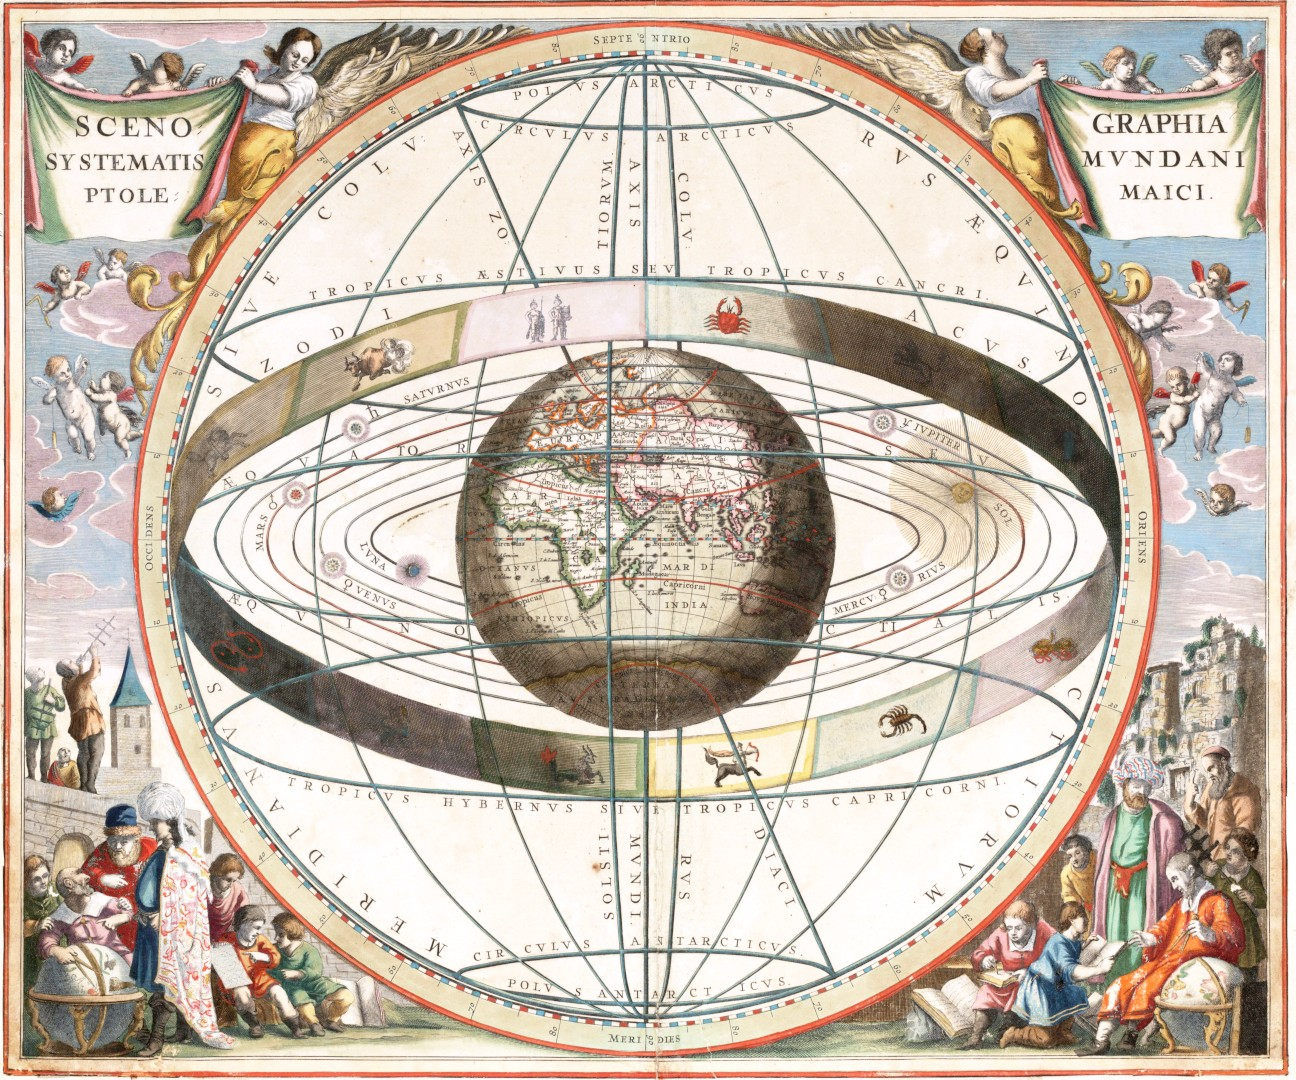
\includegraphics[width=0.8\linewidth]{img/Cellarius_ptolemaic_system}
    \caption{El sistema ptolemaico, en el que la Tierra es el centro del
        universo. Crédito: Loon, J. van (Johannes), aprox. 1611--1686.}
    \label{fig:ptolemaico}
\end{figure}

\subsection*{La revolución científica}
\label{sub:larevolucioncientifica}
Fue hasta 1542 cuando el canónigo católico \index{Copérnico, Nicolás}%
{Nicolás Copérnico} (1473--1543) se atrevió a desafiar el aristotelismo
publicando su libro \emph{De revolutionibus orbium coelestium} (Sobre las
revoluciones de las esferas celestes), en el que propone que el Sol está fijo en
el centro del universo y que los planetas giran alrededor de él, dando lugar así
a la \index{teoría!heliocéntrica}{\emph{teoría heliocéntrica}}.

La teoría no fue bien recibida por la Iglesia, ni aún cuando su autor la dedicó
al Papa Pablo \textsc{iii}.
Más bien fue vetada de 1616 a 1835, pero en solo cien años se había convertido
en la teoría dominante gracias a los trabajos de \index{Galileo Galilei}{Galileo
    Galilei} (1564--1642) y \index{Johannes Kepler}{Johannes Kepler}
(1571--1630).
Kepler descubrió que los planetas se mueven en órbitas elípticas y no circulares
como creía Copérnico, y así resolvió el problema de la posición de Marte en el
cielo nocturno.
En cambio, Galileo apuntó su telescopio al cielo y descubrió que Júpiter tiene
cuatro lunas, que la Luna tiene montañas y cráteres, y que el Sol tiene manchas
entre otras cosas.

Galileo también hizo importantes contribuciones en otras áreas de la ciencia;
descubrió la \emph{ley de caída de los cuerpos}, que dice que todos los cuerpos
caen con la misma aceleración.
Según relata su discípulo Vivianni, esto lo demostró dejando caer dos bolas de
diferente peso desde lo alto de la Torre inclinada de Pisa
\cite{Viviani+2019+1+94}.
Hasta entonces la lógica aristotélica era suficiente para explicar el mundo, la
experimentación era considerada una actividad de segunda clase, y las
matemáticas servían para describir objetos ideales pero no la realidad.
Galileo cambió todo esto, y por ello se le considera el primer científico
moderno.
Desafortunadamente, Galileo fue condenado por la Inquisición en 1633 por
defender a la teoría heliocéntrica, que para entonces era considerada herética
por contradecir la creación del mundo descrita en la Biblia.
Él pasó el resto de su vida bajo arresto domiciliario y se convirtió así también
en el ejemplo más famoso del conflicto entre ciencia y religión.

Luego de la muerte de Galileo, la ciencia entró en una etapa de rápido avance.
\index{Descartes, René}{René Descartes} (1596--1650), con su
\terminology[mecanicismo]{mecanicismo}, propuso que el universo es como una
maquinaria de reloj en la que todo puede explicarse en términos del movimiento
y colisión de partículas.
Asimismo, en su \emph{Discurso del método} (1637) propuso que la ciencia debe
basarse en la razón y no en la autoridad, y que la experimentación y la
observación son las herramientas más importantes para el científico.

Por su parte, \index{Newton, Isaac}{Isaac Newton} (1643--1727) propuso sus tres
leyes del movimiento y la ley de la gravitación universal, que explica la
atracción entre los cuerpos celestes.
Su obra maestra intitulada \emph{Philosophiae Naturalis Principia Mathematica}
(Principios matemáticos de la filosofía natural) se publicó en 1687, y fue el
marco teórico de referencia para la ciencia durante los siguientes 200 años.
Esta teoría sería extendida por muchos otros científicos para explicar más
fenómenos, como la mecánica de fluidos o la teoría electromagnética.

\begin{figure}[ht]
    \centering
    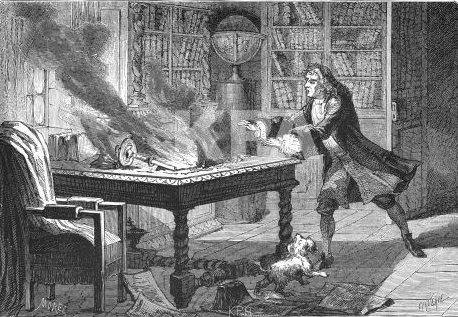
\includegraphics[width=0.8\linewidth]{img/Isaac_Newton_laboratory_fire}
    \caption{Isaac Newton en su laboratorio.
        Su mascota \emph{Diamond} tiró una vela sobre una mesa de papeles,
        quemando varios años de trabajo en el proceso.
        Crédito: Morel / Dominio público.
    }

\end{figure}

Durante un par de siglos se consideró que la teoría de Newton era esencialmente
correcta, y que los científicos sólo necesitaban rellenar meros detalles
técnicos para completar el cuadro.

\subsection*{La ciencia moderna}
\label{sub:lacienciamoderna}
En 1859, \index{Darwin, Charles}{Charles Darwin} (1809--1882) publicó su libro
\emph{El origen de las especies}, en el que propone la teoría de la evolución
mediante la selección natural.
Antes de esto ya se sabía que las especies cambian con el tiempo si se
seleccionan artificialmente a los individuos más aptos para la reproducción.
Así, en la agricultura y la ganadería se habían obtenido nuevas variedades de
plantas y animales más aptas para el consumo humano.
Darwin propuso que este mismo proceso ocurre en la naturaleza, donde las
especies co-evolucionan con su entorno y se adaptan a él.

A mediados del siglo \textsc{xix} el físico escocés \index{Maxwell, James}%
{James Maxwell} (1831--1879) descubrió que la luz es una onda electromagnética
que se propaga a la velocidad de la luz, unificando así las teorías de la
electricidad y el magnetismo.
Esto fue un gran avance, pero también un problema, pues las ecuaciones de
Maxwell entran en conflicto con la mecánica Newtoniana cuando se consideran
altas velocidades.
El final del siglo \textsc{xix} y el principio del \textsc{xx} fueron testigos
de invenciones increíbles como el teléfono, la radio, y el avión, pero también
de descubrimientos científicos que cimbraron la visión mecanicista del mundo.
En 1905, \index{Einstein, Albert}{Albert Einstein} (1879--1955) publicó su
\emph{teoría de la relatividad especial}, en la que propuso que el tiempo y el
espacio son relativos, y que la velocidad de la luz es la misma para todos los
observadores.

Por otro lado, apareció el problema de la \emph{radiación del cuerpo opaco}, que
desafiaba la física clásica al intentar comprender cómo un objeto caliente emite
radiación electromagnética.
Las predicciones clásicas indicaban que bajo ciertas condiciones este emitiría
radiación infinita, en clara contradicción con las observaciones experimentales.
Este problema fue resuelto por \index{Planck, Max}{Max Planck} (1858--1947) en
1900, quien propuso que la energía se emite en paquetes discretos llamados
\emph{cuantos}, dando origen a la \index{mecánica cuántica}{mecánica cuántica}.

En conjunto, la teoría de la relatividad y la mecánica cuántica revolucionaron
la física y la ciencia en general, disminuyendo la confianza en la teoría de
Newton y en el método científico clásico.
Ambas teorías son tan extrañas como exitosas, y han sido confirmadas por miles
de experimentos, pero aún así son difíciles de entender y de aceptar.

En 1936, \index{Turing, Alan}{Alan Turing} (1912--1954) publicó su artículo
\emph{On computable numbers, with an application to the Entscheidungsproblem},
en el que propuso un concepto matemático que eventualmente se convertiría en el
fundamento teórico de la computadora programable.
Su trabajo fue fundamental para el desarrollo de las computadoras y de la
computación moderna, sembrando la posibilidad de analizar a-priori el
comportamiento de un programa de computadora y sus limitaciones, aunque pasarían
varios años antes de que esto se hiciera realidad con la primera computadora
electrónica \emph{ENIAC} (Electronic Numerical Integrator and Computer) en 1946.

Para 1953, \index{Watson, James}{James Watson} (1928--) y
\index{Crick, Francis}{Francis Crick} (1916--2004) descubrieron la estructura
del \index{ácido desoxirribonucleico}{ácido desoxirribonucleico} (ADN), la
molécula que contiene la información genética de los seres vivos, dando inicio
a la \index{biología!molecular}{biología molecular} que estudia los procesos
biológicos en términos de las moléculas que los componen.
Esta disciplina se ha desarrollado rápidamente gracias a la computación, que
permite simular y analizar los procesos biológicos a nivel molecular.
En 2003 se completó el \index{Proyecto Genoma Humano}{Proyecto Genoma Humano},
que consistió en secuenciar el ADN de un ser humano, y que ha permitido
entender mejor las enfermedades genéticas y desarrollar nuevos tratamientos
médicos.

\begin{figure}[ht]
    \centering
    \includegraphics[height=0.618\textheight]%
    {img/60_Jahre_DNA_01.jpg}
    \caption{Réplica del modelo de ADN de Watson y Crick.
        Crédito: Museum für Naturkunde Berlin.}
\end{figure}

\subsection*{La ciencia contemporánea}
El siglo \textsc{xx} fue testigo de la creación o formalización de disciplinas
como \index{economía}{economía}, \index{antrolopogía}{antropología},
\index{sociología}{sociología}, \index{psicología}{psicología}, y
\index{lingüística}{lingüística}.
En general, estas disciplinas se basan en el método científico, pero no son
ciencias naturales.
Por ejemplo, la sociología estudia la sociedad y la cultura, pero es mayormente
una ciencia observacional, pues no se pueden hacer experimentos con sociedades
humanas.

La tendencia actual es hacia la interdisciplinariedad, es decir, la
colaboración entre diferentes disciplinas para resolver un problema.
Una de estas ciencias artificiales que ha contribuido significativamente a
lograr esto es la \index{computación}{computación}, que estudia los fundamentos,
limitaciones y aplicaciones de la programación de computadoras.
La computación ha permitido simular y analizar fenómenos complejos que antes
eran inaccesibles.
Por ejemplo, la climatología estudia el clima de la Tierra, y para ello
simula el comportamiento de la atmósfera mediante modelos computacionales.
Estos métodos computacionales cuestionan la naturaleza misma de la ciencia.
¿Es válido un conocimiento científico que no se basa en la experimentación ni
en la observación, pero que es capaz de predecir el comportamiento de un
fenómeno observado?

Asimismo, la computación ha permitido el desarrollo de la inteligencia
artificial, que estudia la creación de máquinas inteligentes.
Esto ha llevado a la creación de programas de computadora que pueden jugar
ajedrez, conducir automóviles, diagnosticar enfermedades, pero más importante
para nuestra discusión, que hacer ciencia.
Estos programas de computadora se han usado exitosamente para descubrir
exoplanetas, predecir la estructura de proteínas, y descubrir nuevos materiales
entre otras cosas.
¿Se puede considerar \emph{conocimiento científico} a los resultados de estos
programas de computadora?

\section{Qué es la Ciencia}
\label{sec:queeslaciencia}

La ciencia intenta explicar, entender y predecir el mundo que nos rodea, pero
también la religión, la astrología, e incluso otras disciplinas académicas como
la historia y la filosofía.
La diferencia crucial está en los métodos, a saber: la experimentación,
observación y construcción de teorías, pero definir exactamente qué es la
ciencia es un problema que ha ocupado a los filósofos desde hace siglos, este se
conoce como el \terminology[problema!demarcación]{problema de demarcación}.

\subsection{El falsacionismo}
\label{sub:elfalsacionismo}
El filósofo de la ciencia \index{Popper, Karl}{Karl Popper} (1902--1994)
intentó abordar este problema con el \terminology[falsacionismo]{falsacionismo}.
Según Popper, una teoría científica es aquella que, al menos en principio, puede
ser refutada mediante la experimentación.


\section{Los métodos científicos}
\label{sec:losmetodoscientificos}

\section{Las revoluciones científicas}
\label{sec:lasrevolucionescientificas}

\section{Crítica a la ciencia}
\label{sec:criticaalaciencia}
